\documentclass[handout]{beamer}
% \documentclass{beamer}

%%
%%
%%
% From http://tex.stackexchange.com/questions/2072/beamer-navigation-circles-without-subsections
% Solution #2 or 3:
% \usepackage{etoolbox}
% \makeatletter
% % replace the subsection number test with a test that always returns true
% \patchcmd{\slideentry}{\ifnum#2>0}{\ifnum2>0}{}{\@error{unable to patch}}%
% \makeatother
% Solution #1:
\usepackage{remreset}% tiny package containing just the \@removefromreset command
\makeatletter
%\@removefromreset{subsection}{section}
%\makeatother
%\setcounter{subsection}{1}




\usepackage{etex}
\usepackage{pgf}
\usepackage{tikz}
\usepackage{url}
\usepackage{amsmath}
\usepackage{color}
% \definecolor{red}{rgb}{1,0,0}
\usepackage{ulem}
% \usepackage{booktabs}
\usepackage{colortbl,booktabs}
\renewcommand*{\thefootnote}{\fnsymbol{footnote}}
\usepackage{fancybox}
\usepackage[framemethod=TikZ]{mdframed}
\mdfdefinestyle{FactStyle}{%
  outerlinewidth=0.5,
  roundcorner=1pt,
  leftmargin=1cm,
  linecolor=blue,
  outerlinecolor=blue!70!black,
  backgroundcolor=yellow!40
}
\usepackage{cancel}

  \newcommand\Warning{%
    \makebox[2.4em][c]{%
      \makebox[0pt][c]{\raisebox{.2em}{\Large!}}%
      \makebox[0pt][c]{\color{red}\Huge$\bigtriangleup$}}}%

\usepackage{stackengine}
\usepackage{scalerel}
\usepackage{xcolor}
  \newcommand\dangersign[1][2ex]{%
    \renewcommand\stacktype{L}%
    \scaleto{\stackon[1.3pt]{\color{red}$\triangle$}{\tiny !}}{#1}%
  }



\usepackage{dcolumn}
\newcolumntype{d}[1]{D{.}{.}{#1}}

% From
% http://tex.stackexchange.com/questions/109900/how-can-i-box-multiple-aligned-equations
\usepackage{empheq}
\usepackage{tcolorbox}  \newtcbox{\othermathbox}[1][]{%
  nobeforeafter, tcbox raise base, 
  colback=black!10, colframe=red!30, 
  left=1em, top=0.5em, right=1em, bottom=0.5em}

\newcommand\blue{\color{blue}}
\newcommand\red{\color{red}}
\newcommand\green{\color{green!75!black}}
\newcommand\purple{\color{purple}}
\newcommand\bluegreen{\color{blue!75!green}}
\newcommand\orange{\color{orange}}
\newcommand\redgreen{\color{red!50!green}}
\newcommand\grey{\color{black}}
\newcommand\gap{\vspace{.1in}}
\newcommand\nb{${\red\bullet}\ $}
\newcommand\halfgap{\vspace{.05in}}
\newcommand\divideline{\line(1,0){352}}
\usepackage{marvosym} % for \Smiley

\newcommand{\bluealert}[1]{{\blue\textbf{#1}}}

% \usepackage{beamerthemesplit} %Key package for beamer
\usetheme{Singapore}
% \usetheme{Szeged}
% \usetheme{Garfield}
% \usetheme{CambridgeUS}
% \usenavigationsymbolstemplate{} %Gets rid of slide navigation symbols


\setbeamercolor{separation line}{use=structure,bg=structure.fg!50!bg}
% \begin{beamercolorbox}[colsep=0.5pt]
%   {upper separation line foot}
% \end{beamercolorbox}



\makeatletter
\setbeamertemplate{footline}
{
  \leavevmode%
  \hbox{%
% \begin{beamercolorbox}[colsep=0.5pt]
%   {upper separation line foot}
% \end{beamercolorbox}


  \begin{beamercolorbox}[wd=.5\paperwidth,ht=2.25ex,dp=2ex,colsep=0.5pt]%
    {upper separation line foot}
    \usebeamerfont{author in head/foot}%
    \hspace*{2ex}\insertshortdate:\ \insertshorttitle
  \end{beamercolorbox}%
  \begin{beamercolorbox}[wd=.5\paperwidth,ht=2.25ex,dp=2ex,right]{title in head/foot}%
    \usebeamerfont{title in head/foot}
    {\insertshortauthor}\hspace*{2ex}
  \end{beamercolorbox}}%
  % \begin{beamercolorbox}[wd=.333333\paperwidth,ht=2.25ex,dp=2ex,right]{date in head/foot}%
  %   \usebeamerfont{date in head/foot}\insertshortdate{}\hspace*{2em}
  %   \insertframenumber{} / \inserttotalframenumber\hspace*{2ex} 
  % \end{beamercolorbox}%
  \vskip0pt%
}
\makeatother

\usetikzlibrary{decorations.markings}
\usetikzlibrary{arrows}


\title{Final Exam Review}
\author{Schley, UCSB Mathematics}
\date{March 15, 2017}
%\institute{}


\useinnertheme{default}

\usefonttheme{serif}
% \usecolortheme{rose}
% \usecolortheme{whale}
% \usecolortheme{orchid}
\usecolortheme{crane}
% \usecolortheme{dolphin}


%TEMPLATE
\setbeamertemplate{navigation symbols}{}

\setbeamertemplate{note page}[compress]

\setbeamertemplate{frametitle}{
  \vspace{0.5em}
  % \begin{centering}
  {\huge\blue\textbf{\textmd{\insertframetitle}}}
  \par
  % \end{centering}
}

% From http://tex.stackexchange.com/questions/7032/good-way-to-make-textcircled-numbers:
\newcommand*\circled[1]{\tikz[baseline=(char.base)]{\node[shape=circle,draw,fill=orange,inner sep=1pt] (char) {#1};}} 
% \renewcommand{\labelenumi}{\circled{\textbf{\arabic{enumi}}}}

\let\olddescription\description
\let\oldenddescription\enddescription
\usepackage{enumitem}
\let\description\olddescription
\let\enddescription\oldenddescription

% \usepackage[loadonly]{enumitem}
\setlist[enumerate,1]{label=\colorbox{orange}{\arabic*.},font=\bfseries}
%\setlist[enumerate,2]{label=\colorbox{blue!25}{(\alph*)},font=\bfseries}
% \setlist[enumerate,1]{label=\arabic*.,font=\bfseries}
\setlist[itemize,1]{label=\red$\bullet$}
\setlist[itemize,2]{label=\blue$\bullet$}

\newcommand\answer[1]{\fbox{#1}}
% \renewcommand\answer[1]{}

\newcommand{\antilog}{\operatorname{antilog}}

\newcommand{\instructor}{Nathan Schley ({\it Sh}+{\it lye})}
\newcommand{\officehours}{T R 11-11:50, T 3:45-4:35 Details on Gauchospace.}
\newcommand{\email}{schley@math.ucsb.edu}
\newcommand{\officeloc}{South Hall 6701}
\newcommand{\copyrightinfo}{2022\ Daryl Cooper, Peter M.\ Garfield, Ebrahim Ebrahim \& Nathan Schley}
    













\title{}
\title{Cool Stuff With Lines}
\date{April 17, 2017}


\begin{document}
\small

\section*{Administration}

\frame{
  \frametitle{Office Hours!}
  % \ \vspace*{0.25in}

  {\Large{}Instructor:}\\
  \ \hspace*{0.2in} Peter M.\ Garfield, \url{garfield@math.ucsb.edu}\\[0.25em]

  {\Large{}Office Hours:}\\
  \ \hspace*{0.2in} Mondays 1--2\textsc{pm}\\
  \ \hspace*{0.2in} Tuesdays 10:30--11:30\textsc{am}\\
  \ \hspace*{0.2in} Thursdays 1--2\textsc{pm}\\
  \ \hspace*{0.2in} or by appointment \\[0.25em]

  {\Large{}Office:}\\
  \ \hspace*{0.2in} South Hall 6510\\[0.5em]

  \copyright\ 2017\ Daryl Cooper, Peter M.\ Garfield

  % \vspace*{2in}
}

\section*{Proportionality}

\frame{
  \frametitle{Proportionality Review}

  
  ``$y$ is proportional to $x$'' or $y\propto x$ means
  \begin{itemize}
  \item When we double $x$, we double $y$
    \pause

  \item When we triple $x$, we triple $y$
    \pause

  \item When we halve $x$, we halve $y$
    \pause

  \item $y=Kx$, where $K$ is called the
  \alert{\emph{constant of proportionality}}. 

  \end{itemize}

  \vspace*{1in}



}

\frame{
  \frametitle{Constant of Proportionality}

  \alert{Example:}\ We are told
  \begin{itemize}
  \item Tax is proportional to income, and 
  \item The tax on \$$1,000$\ is \$$280$.
  \end{itemize}
  Express $y = \text{amount of tax paid}$\ in terms of  $x = \text{the
    income}$. Then $y=$
  \begin{center}
    \mbox{
      A$= 1000x$
      \quad 
      B$= 280x$
      \quad 
      C$=\dfrac{1,000}{280}\,x$
    }
    \\[0.5em]
    \mbox{
      D$=2.8x$
      \quad 
      E$= 0.28x$
      \pause
      \quad 
      \answer{E} 
    }
  \end{center}
  \gap

  \alert{Question:}\ What does the constant of proportionality
  $K=0.28$ mean?
  \pause\halfgap

  \alert{Answer:}\ It is the tax on one dollar.


}


\frame{
  \frametitle{Example}

  For this question, we assume:
  \begin{itemize}
  \item   The weight of an elephant is proportional to its
    \alert{\emph{height cubed}}, and

  \item   An elephant 1 meter high weighs $1/3$ tons. 
  \end{itemize}

  How many tons does an elephant $h$ meters tall weigh?
  \begin{center}
    A$= h/3$
    \quad 
    B$= h^3$
    \quad 
    C$ = h^3/3$
    \quad 
    D$ = (h/3)^3$
    \quad 
    E$ = (3h)^3$
    \pause
    \quad
    \answer{C}
  \end{center}
  \gap

  \alert{Question:}\ What does the constant of proportionality
  $K=1/3$ mean?
  \pause\halfgap

  \alert{Answer:}\ It is the weight of $1$ cubic meter of elephant.

}

\frame{
  \frametitle{More Complicated Examples}
  
  \begin{empheq}[box=\othermathbox]{equation*}
    \text{$y$ is \alert{inversely proportional} to $x$ means $y\propto 1/x$}
  \end{empheq}
  \pause

  Example:
  \begin{itemize}
  \item I have \$$300$
  \item $N=$ number of apples I can buy
  \item $p=$ price per apple
  \end{itemize}
  Then $N$ is inversely proportional to $p$: $N\propto 1/p$.
  \bigskip
  \pause

  \alert{Question:}\ What is the constant of proportionality?
  \smallskip
  \pause

  \alert{Answer:}\ It is \$$300$, the amount of money I have.
  \gap

}

\frame{
  \frametitle{More Complicated Examples}
  
  \begin{empheq}[box=\othermathbox]{equation*}
    \text{$z$ is \alert{jointly proportional} to $x$ and $y$ means $x\propto
      x\cdot y$ (or $z=Kxy$)}
  \end{empheq}
  \pause

  Example:
  \begin{itemize}
  \item $C =$ cost of a rectangular plot of land,
  \item $\ell=$ length (in meters) of plot, and
  \item $w=$ width (in meters) of plot.
  \end{itemize}
  Then $C$ is jointly proportional to $\ell$ and $w$: $C=K\cdot \ell
  \cdot w$.
  \bigskip
  \pause

  \alert{Question:}\ What does the constant of proportionality mean?
  \pause
  \smallskip

  \alert{Answer:}\ It is the cost of one square meter of land.



}

\frame{
  \frametitle{More Complicated Examples}

  \alert{\large{}Strength of Light}\
  \begin{itemize}
  \item $P\;$\parbox[t]{2.5in}{%
      $=\text{strength of light (\colorbox{yellow}{power}\ per unit area)}$ \\
      \pause%
      $=\text{amount of light on unit area}$
    }
    \pause

  \item $R = $ distance to light source
    \pause
  \end{itemize}
  \gap

  \alert{Inverse Square Law:}\ $P\propto 1/R^2$
  \pause
  \gap

  Same idea for heat, gravity, sound, and many others\ldots
  \pause
  \gap

  \alert{Newton's Law of Gravity:}\ $F \propto \dfrac{m_1m_2}{r^2}$
  \pause
  \halfgap

  Constant of proportionality: 
  \parbox[t]{2in}{%
    $G\approx 6.67\times 10^{-11}\ \text{m}^3/(\text{kg}\,\cdot\,
    \text{s}^{2})$\\[0.25em]
    (the \colorbox{yellow}{Gravitational constant})
  }

}

\section*{Review}

\frame{
  \frametitle{Winter 17 Exam \#1}

  \begin{enumerate}
  \item Solve for $x$ in the equation
    \begin{equation*}
      \frac{3}{x+a} = \frac{a}{x+2}.
    \end{equation*}
    \vspace*{0.5in}
    \pause

  \item Multiply out and simplify.  Check your answer.
    \begin{equation*}
      (a-3b)(4a+2b) + 6ab
    \end{equation*}
    \vspace*{0.5in}
  \end{enumerate}

}

\frame{
  \frametitle{Winter 17 Exam \#1}

  \begin{enumerate}
    \setcounter{enumi}{2}
  \item Substitute $x=3t-4$\ into
    \begin{equation*}
      2x(x+1).
    \end{equation*}
    Simplify the result as much as possible. 
    \vspace*{0.5in}
    \pause

  \item Solve for $x$ and $y$ in the simultaneous equations
    \begin{equation*}
      x+2y=p
      \qquad\qquad
      x+y=4.
    \end{equation*}
    \vspace*{0.5in}
  \end{enumerate}
}


\frame{
  \frametitle{Winter 17 Exam \#1}

  \begin{enumerate}
    \setcounter{enumi}{4}
  \item Marie leaves Santa Barbara at 10am, driving to Bakersfield on
    a route which is $150$\ miles\ long.  Jason leaves Bakersfield at
    11am driving the same route to Santa Barbara.  Marie's speed is
    $40\ \text{miles}/\text{hr}$\ and Jason's speed is
    $60\ \text{miles}/\text{hr}$.
    \vspace*{0.2in}
    \begin{enumerate}
      \item[\colorbox{blue!25}{(a)}] How far apart are they at noon?
        \vspace*{0.2in}
        \pause

      \item[\colorbox{blue!25}{(b)}] How far from Santa Barbara are
        they when they meet? 
        \vspace*{0.2in}
        \pause
        
      \item[\colorbox{blue!25}{(c)}] How many hours has \emph{Jason}\
        been driving when they meet?\\ 
        {\tiny[leave your answers as \emph{fractions}]}
        \vspace*{0.2in}

    \end{enumerate}
  \end{enumerate}
}

\frame{
  \frametitle{Winter 17 Exam \#1}

  \begin{enumerate}
    \setcounter{enumi}{5}
  \item A farmer wants to partition a rectangular field into quarters,
    as shown.  The total area of the field is $500$\ square
    meters. Suppose the length of the field is $L$ meters.

    \begin{minipage}[t]{0.450\linewidth}
      \begin{enumerate}
      \item[\colorbox{blue!25}{(a)}] Express the width of the field in
        terms of $L$. \\[0.5em] 
      \end{enumerate}
    \end{minipage}
    \begin{minipage}[t]{0.50\linewidth}
      \begin{center}
        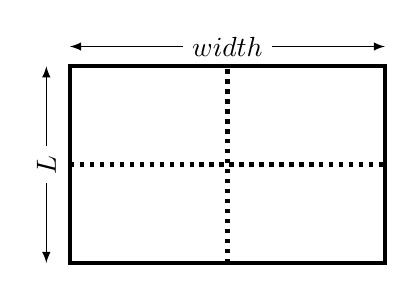
\begin{tikzpicture}[x=10mm,y=25mm,>=latex,baseline=25mm]
          \draw[thin,black,<->] (-0.3,0) -- (-0.3,1) node[midway,fill=white,rotate=90] {$L$};
          \draw[thin,black,<->] (0,1.1) -- (4,1.1) node[midway,fill=white] {$width$};
          \draw[ultra thick,black] (0,0) rectangle (4,1);
          \draw[ultra thick,black,dotted] (0,0.5) -- (4,0.5);
          \draw[ultra thick,black,dotted] (2,0) -- (2,1);
        \end{tikzpicture}
      \end{center}
    \end{minipage}
    % \bigskip
    \begin{enumerate}
      \item[\colorbox{blue!25}{(b)}] 
      The outer boundary fence (on the perimeter of the field, shown solid)
      costs \$$4$ per meter, and the inside fence (shown dotted) costs
      \$$3$ per meter. Express the total cost of the fence needed in terms
      of $L$.
      % Express the total number of meters of fence needed in terms of $L$.
      % \bigskip
    \end{enumerate}
  \end{enumerate}



}



\end{document}


%%% Local Variables: 
%%% mode: latex
%%% TeX-master: t
%%% End: 
